%%
%% This is file for CAIS 2026 submission
%% ACM Conference on AI and Agentic Systems
%%

\documentclass[sigconf,review,anonymous]{acmart}

%% Rights management information
\setcopyright{acmlicensed}
\copyrightyear{2026}
\acmYear{2026}
\acmDOI{XXXXXXX.XXXXXXX}

%% Conference information
\acmConference[CAIS '26]{ACM Conference on AI and Agentic Systems}{May 26--29, 2026}{San Jose, CA, USA}
\acmBooktitle{Proceedings of the ACM Conference on AI and Agentic Systems (CAIS '26), May 26--29, 2026, San Jose, CA, USA}
\acmISBN{978-1-4503-XXXX-X/26/05}

%% Packages
\usepackage{booktabs}
\usepackage{amsmath}
\usepackage{graphicx}
\usepackage{listings}
\usepackage{xcolor}
\usepackage{tikz}
\usetikzlibrary{shapes.geometric, arrows.meta, positioning, fit, backgrounds, calc}

%% TikZ styles
\tikzset{
  sysblock/.style={rectangle, draw, fill=blue!8, text width=2.2cm, minimum height=0.9cm, align=center, rounded corners=2pt, font=\small},
  pillarbox/.style={rectangle, draw, fill=orange!12, text width=2cm, minimum height=0.8cm, align=center, rounded corners=2pt, font=\small\bfseries},
  procbox/.style={rectangle, draw, fill=green!8, text width=2cm, minimum height=0.7cm, align=center, rounded corners=2pt, font=\small},
  databox/.style={trapezium, trapezium left angle=70, trapezium right angle=110, draw, fill=yellow!10, text width=1.6cm, minimum height=0.6cm, align=center, font=\small},
  arr/.style={-{Stealth[length=2.5mm]}, thick},
  darr/.style={-{Stealth[length=2.5mm]}, thick, dashed},
}

%% Code listing style
\lstset{
  basicstyle=\ttfamily\small,
  breaklines=true,
  frame=single,
  backgroundcolor=\color{gray!10}
}

%%
%% Document starts
%%
\begin{document}

%%
%% Title
%%
\title{Closing the Feedback Loop: Iterative Agent Tooling Improvement Through Trajectory Analysis and Agentic DevX Metrics}

%%
%% Authors (anonymous for review)
%%
\author{Anonymous Authors}
\affiliation{%
  \institution{Anonymous Institution}
}
\email{anonymous@example.com}

%%
%% Abstract
%%
\begin{abstract}
When AI agents fail to build production applications, should we improve the agent or its environment? Recent work suggests that environment quality---templates, tools, guidance---matters more than model selection~\cite{kniazev2025appbuild}. We present a feedback loop for iterative tooling improvement: (1)~an \textbf{installable domain knowledge} architecture packages expertise as agent-consumable artifacts; (2)~agents use this package to generate applications, producing execution trajectories; (3)~an \textbf{agentic trajectory analyzer} processes these trajectories to identify friction and recommend fixes to the package; (4)~\textbf{Agentic DevX metrics} serve as the final quality gate, measuring whether generated applications can be operated by other agents. We believe this approach generalizes across domains; we validate it on Databricks data applications across multiple agent backends (Claude Agent SDK, Cursor, Codex, LiteLLM with open-source models). On 20 applications, we achieve 90\% one-shot build success at \$0.74/app. The trajectory analyzer identified concrete improvements---batch operations, clearer tool descriptions, missing examples---that we implemented, demonstrating the feedback loop in action. The architecture is designed for automatic optimization: the analyzer's recommendations target tool descriptions, prompts, and examples---artifacts amenable to techniques like GEPA or DSPy-style prompt tuning, potentially closing the loop without human intervention.
\end{abstract}

%%
%% CCS Concepts
%%
\begin{CCSXML}
<ccs2012>
   <concept>
       <concept_id>10011007.10011006.10011008.10011009.10011015</concept_id>
       <concept_desc>Software and its engineering~Software testing and debugging</concept_desc>
       <concept_significance>500</concept_significance>
   </concept>
   <concept>
       <concept_id>10010147.10010178.10010179</concept_id>
       <concept_desc>Computing methodologies~Natural language processing</concept_desc>
       <concept_significance>300</concept_significance>
   </concept>
</ccs2012>
\end{CCSXML}

\ccsdesc[500]{Software and its engineering~Software testing and debugging}
\ccsdesc[300]{Computing methodologies~Natural language processing}

%%
%% Keywords
%%
\keywords{agent-agnostic tooling, agentic code generation, trajectory analysis, developer experience metrics, feedback loop}

\maketitle

%% ============================================================
%% 1. INTRODUCTION
%% ============================================================
\section{Introduction}
\label{sec:intro}

AI agents can generate functional software, but they lack domain-specific knowledge required for production applications. The conventional response is building better agents. We take a different approach: improve what agents have access to.

This approach is motivated by recent findings~\cite{kniazev2025appbuild}: when comparing agent performance across environments while holding the model constant, environment quality (templates, tools, guidance) had larger effects than model upgrades. An agent with excellent tooling outperforms a better model with poor tooling.

Accepting that tooling matters raises a question: how do we improve it systematically? Manual inspection doesn't scale. End-state metrics (build pass/fail) don't reveal causes. We need a feedback loop that:

\begin{enumerate}
    \item Captures how agents actually use tooling (trajectories)
    \item Identifies friction points and root causes (analysis)
    \item Produces actionable recommendations (fixes)
    \item Verifies improvements against agent-centric criteria (evaluation)
\end{enumerate}

%% --- TikZ Figure 1: System Overview / Feedback Loop ---
\begin{figure}[t]
\centering
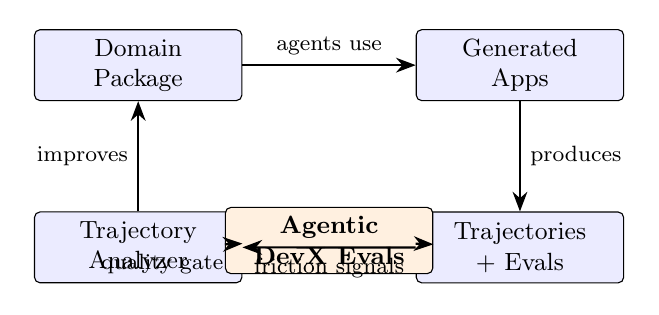
\begin{tikzpicture}[node distance=1.4cm and 1.8cm]
  % Nodes
  \node[sysblock, text width=2.4cm] (pkg) {Domain\\Package};
  \node[sysblock, text width=2.4cm, right=2.2cm of pkg] (apps) {Generated\\Apps};
  \node[sysblock, text width=2.4cm, below=of apps] (traj) {Trajectories\\+ Evals};
  \node[sysblock, text width=2.4cm, below=of pkg] (analyzer) {Trajectory\\Analyzer};
  \node[pillarbox, text width=2.4cm, below=1.8cm of $(pkg)!0.5!(apps)$] (devx) {Agentic\\DevX Evals};

  % Arrows
  \draw[arr] (pkg) -- node[above, font=\footnotesize]{agents use} (apps);
  \draw[arr] (apps) -- node[right, font=\footnotesize]{produces} (traj);
  \draw[arr] (traj) -- node[below, font=\footnotesize]{friction signals} (analyzer);
  \draw[arr] (analyzer) -- node[left, font=\footnotesize]{improves} (pkg);
  \draw[darr] (traj) -- (devx);
  \draw[darr] (devx) -- node[below left, font=\footnotesize]{quality gate} (analyzer);
\end{tikzpicture}
\caption{The feedback loop. Trajectories feed the analyzer, which improves the domain package. Agentic DevX evals verify the final output.}
\label{fig:feedback-loop}
\end{figure}

We instantiate each component (Figure~\ref{fig:feedback-loop}):

\begin{enumerate}
    \item \textbf{Installable Domain Knowledge} (Section~\ref{sec:domain-knowledge}). An architecture for packaging domain expertise as agent-consumable artifacts. We validate on Databricks, exposing tools via CLI commands---applicable to emerging standards like Agent Skills.

    \item \textbf{Agentic Trajectory Analyzer} (Section~\ref{sec:trajectory}). A two-phase system: parallel friction extraction with a cheap model followed by agentic synthesis with a reasoning model that has source code access. The analyzer consumes trajectories and optionally evaluation results.

    \item \textbf{Agentic DevX Metrics} (Section~\ref{sec:devx}). The final quality gate: Runability (0--5) and Deployability (0--5) measure whether another agent---not a human---can operate generated applications. This is a novel evaluation dimension absent from existing benchmarks.
\end{enumerate}

\textbf{Validation.} We validate across Claude Agent SDK (primary), Cursor, Codex (manual), and LiteLLM with open-source models. On 20 Databricks applications: 90\% build success, 90\% database connectivity, \$0.74/app, 6--9 minute latency. The trajectory analyzer identified improvements that we implemented and verified through multiple iterations.

%% ============================================================
%% 2. INSTALLABLE DOMAIN KNOWLEDGE
%% ============================================================
\section{Installable Domain Knowledge}
\label{sec:domain-knowledge}

\subsection{Motivation}
\label{sec:dk-motivation}

Developers already use capable agents---Claude Code, Cursor, Codex. Rather than asking them to adopt yet another tool, we bring domain knowledge to the agents they already use. A user installs our package into their existing environment; the agent gains domain expertise without workflow changes.

This approach has a practical advantage: we leverage the ecosystem of existing agents rather than competing with them. The alternative---building a custom agent per domain---doesn't scale and creates vendor lock-in.

\subsection{Architecture}
\label{sec:dk-architecture}

The package has three components: context layers that inject domain knowledge progressively, tools exposed via CLI, and a state machine that enforces validation before deployment.

%% --- TikZ Figure 2: Domain Package Architecture ---
\begin{figure}[t]
\centering
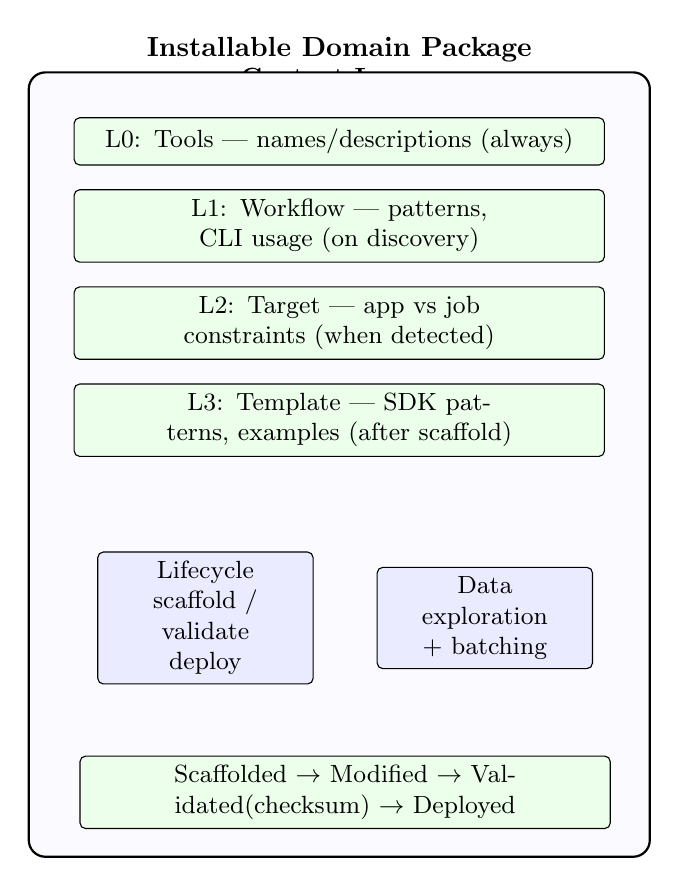
\begin{tikzpicture}[node distance=0.6cm]
  % Context layers
  \node[procbox, text width=6.5cm, minimum height=0.6cm] (l0) {L0: Tools --- names/descriptions (always)};
  \node[procbox, text width=6.5cm, minimum height=0.6cm, below=0.3cm of l0] (l1) {L1: Workflow --- patterns, CLI usage (on discovery)};
  \node[procbox, text width=6.5cm, minimum height=0.6cm, below=0.3cm of l1] (l2) {L2: Target --- app vs job constraints (when detected)};
  \node[procbox, text width=6.5cm, minimum height=0.6cm, below=0.3cm of l2] (l3) {L3: Template --- SDK patterns, examples (after scaffold)};

  % Fit around context layers
  \begin{scope}[on background layer]
    \node[draw, rounded corners=4pt, fill=green!3, fit=(l0)(l3), inner sep=6pt, label={[font=\small\bfseries]above:Context Layers}] (ctx) {};
  \end{scope}

  % Tools
  \node[sysblock, text width=2.5cm, below=1.2cm of l3.south west, anchor=north west, xshift=0.3cm] (lifecycle) {Lifecycle\\scaffold / validate\\deploy};
  \node[sysblock, text width=2.5cm, right=0.8cm of lifecycle] (data) {Data\\exploration\\+ batching};

  % State machine
  \node[procbox, text width=6.5cm, minimum height=0.6cm, below=1.0cm of $(lifecycle.south)!0.5!(data.south)$] (sm) {Scaffolded $\to$ Modified $\to$ Validated(checksum) $\to$ Deployed};

  % Outer box
  \begin{scope}[on background layer]
    \node[draw, thick, rounded corners=6pt, fill=blue!2, fit=(ctx)(lifecycle)(data)(sm), inner sep=10pt, label={[font=\bfseries]above:Installable Domain Package}] {};
  \end{scope}
\end{tikzpicture}
\caption{Domain package architecture. Context layers avoid token overload; the state machine enforces validation before deployment.}
\label{fig:domain-package}
\end{figure}

\subsection{Context Layers}
\label{sec:dk-context}

Agents have limited context windows. Dumping all domain knowledge upfront wastes tokens and can confuse the model. Instead, we inject context progressively---each layer activates when relevant (Figure~\ref{fig:domain-package}).

\begin{table}[h]
\caption{Context layer injection strategy.}
\label{tab:context-layers}
\centering
\small
\begin{tabular}{llp{3.2cm}}
\toprule
\textbf{Layer} & \textbf{Content} & \textbf{When Injected} \\
\midrule
L0: Tools & Tool names/descriptions & Always (protocol-level) \\
L1: Workflow & Patterns, CLI usage & On first discovery call \\
L2: Target & App vs job constraints & When target type detected \\
L3: Template & SDK patterns, examples & After scaffolding or from CLAUDE.md \\
\bottomrule
\end{tabular}
\end{table}

For example, an agent scaffolding a new app receives L0--L2 initially. Only after scaffolding completes does L3 activate---providing SDK-specific patterns like ``how to draw charts with Recharts'' or ``tRPC router conventions''. For existing projects, the agent reads CLAUDE.md (placed in the project root) to acquire L3 context.

\subsection{Tools}
\label{sec:dk-tools}

We expose domain functionality through CLI commands---a pattern that Cloudflare~\cite{cloudflare2024codemode} and Anthropic~\cite{anthropic2024tools} found effective, reporting that LLMs perform better writing code to call tools than calling tools directly.

\textbf{Lifecycle commands:} \texttt{scaffold} (creates project from template with CLAUDE.md guidance), \texttt{validate} (builds in Docker, captures Playwright screenshot), \texttt{deploy} (to target platform).

\textbf{Data exploration:} Commands for discovering available data, with agent-friendly additions: batch operations that bundle multiple queries, clearer error messages, and syntax examples for platform-specific SQL variations.

Workspace tools (read/write/edit, grep, glob, bash) are not our contribution---agents already have these. Our package adds domain-specific capabilities on top.

\subsection{State Machine}
\label{sec:dk-state}

Applications cannot deploy unless they pass validation after their most recent modification:

\begin{center}
\texttt{Scaffolded $\xrightarrow{\text{edit}}$ Modified $\xrightarrow{\text{validate}}$ Validated(checksum) $\xrightarrow{\text{deploy}}$ Deployed}
\end{center}

The checksum captures state at validation time. Any change after validation requires re-validation. This prevents untested code deployment---a common failure mode when agents skip validation.

\subsection{Agent Compatibility}
\label{sec:dk-compat}

To validate agent-agnosticism, we tested the package across multiple backends. The key requirement is function calling capability---any agent that can invoke tools works with our package.

\begin{table}[h]
\caption{Agent backend compatibility validation.}
\label{tab:agent-compat}
\centering
\small
\begin{tabular}{lll}
\toprule
\textbf{Backend} & \textbf{Validation} & \textbf{Notes} \\
\midrule
Claude Agent SDK & Automated & Primary production use \\
Cursor & Manual & IDE integration \\
Codex & Manual & Alternative agent \\
LiteLLM + Qwen3 & Automated & Open-source (70\% at \$0.61/app) \\
\bottomrule
\end{tabular}
\end{table}

The LiteLLM backend demonstrates that the approach isn't tied to specific vendors---we wrap any model with function calling into our generation pipeline.

%% ============================================================
%% 3. AGENTIC TRAJECTORY ANALYZER
%% ============================================================
\section{Agentic Trajectory Analyzer}
\label{sec:trajectory}

\subsection{Role in the Feedback Loop}
\label{sec:ta-role}

To run trajectory analysis at scale, we built infrastructure for bulk app generation that saves execution traces in a structured format. In production, users work with their own agents (Cursor, Claude Code) which may not save trajectories in our format---but the analyzer works with any trace data that captures tool calls and results.

The analyzer consumes trajectories and recommends package improvements. This closes the loop: agents struggle $\rightarrow$ we see it in trajectories $\rightarrow$ we fix the tooling $\rightarrow$ agents struggle less.

\subsection{Why Trajectories, Not Just Outcomes}
\label{sec:ta-why}

End-state metrics (build success, test pass) don't reveal causes:

\begin{itemize}
    \item Model limitations (reasoning, instruction following)?
    \item Tool problems (unclear descriptions, missing functionality)?
    \item Template issues (incorrect scaffolding, missing guidance)?
    \item Prompt issues (underspecified requirements, contradicting constraints)?
\end{itemize}

Trajectories---the sequence of reasoning, tool calls, and results---show where things went wrong. An agent retrying the same malformed SQL five times reveals a missing example. An agent calling N tools for N tables reveals a missing batch operation.

\subsection{Two-Phase Architecture}
\label{sec:ta-architecture}

%% --- TikZ Figure 3: Map-Reduce Trajectory Pipeline ---
\begin{figure}[t]
\centering
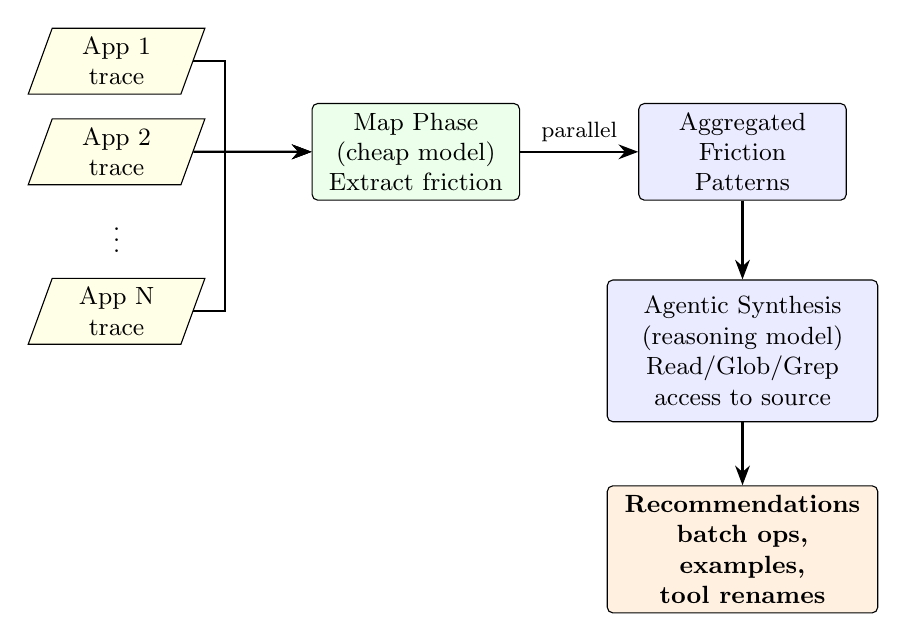
\begin{tikzpicture}[node distance=0.8cm and 1.2cm]
  % Trajectories
  \node[databox, text width=1.4cm] (t1) {App 1\\trace};
  \node[databox, text width=1.4cm, below=0.3cm of t1] (t2) {App 2\\trace};
  \node[below=0.2cm of t2, font=\small] (dots) {$\vdots$};
  \node[databox, text width=1.4cm, below=0.2cm of dots] (tn) {App N\\trace};

  % Map phase
  \node[procbox, text width=2.4cm, right=1.5cm of t2] (map) {Map Phase\\(cheap model)\\Extract friction};

  % Aggregated
  \node[sysblock, text width=2.4cm, right=1.5cm of map] (agg) {Aggregated\\Friction\\Patterns};

  % Synthesis
  \node[sysblock, text width=3.2cm, minimum height=1.8cm, below=1.0cm of agg] (synth) {Agentic Synthesis\\(reasoning model)\\Read/Glob/Grep\\access to source};

  % Recommendations
  \node[pillarbox, text width=3.2cm, below=0.8cm of synth] (rec) {Recommendations\\batch ops, examples,\\tool renames};

  % Arrows
  \draw[arr] (t1.east) -- ++(0.4,0) |- (map.west);
  \draw[arr] (t2) -- (map);
  \draw[arr] (tn.east) -- ++(0.4,0) |- (map.west);
  \draw[arr] (map) -- node[above, font=\footnotesize]{parallel} (agg);
  \draw[arr] (agg) -- (synth);
  \draw[arr] (synth) -- (rec);
\end{tikzpicture}
\caption{Two-phase trajectory analyzer. Map phase extracts friction in parallel; synthesis phase explores source code to find root causes and generate recommendations.}
\label{fig:trajectory-pipeline}
\end{figure}

We employ a map-reduce approach optimized for cost and quality (Figure~\ref{fig:trajectory-pipeline}).

\textbf{Map phase.} Each trajectory is processed independently by a cheap model (we use Claude Haiku, $\sim$\$0.001/trajectory), extracting errors, retries, confusion patterns, and inefficient tool usage. This runs in parallel.

\textbf{Agentic synthesis phase.} Aggregated patterns go to a reasoning model (we use Claude Opus) with read-only access to:
\begin{itemize}
    \item Template and CLI tools source code (via Read/Glob/Grep)
    \item Tool definitions (extracted from MCP server)
    \item Evaluation metrics (per-app scores, optional)
\end{itemize}

This is a full agent with up to 50 turns of exploration. If trajectories show SQL confusion, the agent greps templates for SQL examples. If tool descriptions seem unclear, it reads implementations. Context is discovered progressively as patterns demand.

\textbf{Extensibility.} The architecture naturally extends to new context sources. We started with trajectories only, then added template source code access, then tool definitions extracted via the MCP binary. Adding new sources (e.g., user feedback, production logs) requires only pointing the synthesis agent at additional files.

\subsection{Concrete Improvements}
\label{sec:ta-improvements}

The analyzer identified issues leading to fixes we implemented:

\begin{table}[h]
\caption{Trajectory-identified improvements (implemented).}
\label{tab:improvements}
\centering
\small
\begin{tabular}{p{2.2cm}p{2.2cm}p{2.8cm}}
\toprule
\textbf{Pattern Observed} & \textbf{Diagnosis} & \textbf{Fix Applied} \\
\midrule
N separate calls for N tables & Missing batch operation & Added \texttt{discover\_schema} batch command \\
Agents expecting list, got search & Confusing tool name & Renamed \texttt{list\_tables} $\to$ \texttt{find\_tables} \\
Repeated SQL syntax errors & Missing examples & Added QUALIFY, PIVOT syntax to guidance \\
Retries on malformed errors & Unclear error messages & Added contextual parameter messages \\
\bottomrule
\end{tabular}
\end{table}

These aren't hypothetical---they're actual fixes derived from trajectory analysis and committed to the codebase.

\subsection{Cost Model}
\label{sec:ta-cost}

For $N$ trajectories:
\begin{itemize}
    \item Map: $N \times {\sim}\$0.001$ (cheap model)
    \item Synthesis: $1 \times {\sim}\$0.5$--3 (reasoning model, bounded at 50 turns)
\end{itemize}

Total scales linearly but remains bounded. For 20 apps, analysis cost was under \$15.

\subsection{Future Direction}
\label{sec:ta-future}

Our current approach is semi-automatic: the analyzer outputs recommendations, but a human reviews them and decides which to implement. Recent work on reflective prompt evolution (GEPA~\cite{gepa2024}) and DSPy~\cite{khattab2023dspy} shows prompts can be automatically optimized through self-reflection. The analyzer's recommendations target tool descriptions, prompts, and examples---artifacts amenable to such techniques, potentially closing the loop without human intervention.

%% ============================================================
%% 4. AGENTIC DEVX METRICS
%% ============================================================
\section{Agentic DevX Metrics}
\label{sec:devx}

\subsection{Role in the Feedback Loop}
\label{sec:devx-role}

Agentic DevX is the final quality gate. After the package is improved and agents generate applications, we need to verify: can another agent actually operate this output?

This is distinct from the trajectory analyzer's role. The analyzer improves the package based on how agents behave during generation. DevX metrics evaluate the result---whether generated applications meet agent-operability criteria.

\subsection{Motivation}
\label{sec:devx-motivation}

Consider an agent that generates a working application. A human developer can run it: they'll figure out missing environment variables, install unlisted dependencies, work around unclear documentation. An agent \emph{can sometimes} do this too, but it's slow and inefficient---spending many turns on trial-and-error that explicit configuration would eliminate. It needs explicit \texttt{.env.example} files, documented commands, health endpoints for verification.

Existing metrics miss this distinction. Build success (binary) doesn't capture whether the build process is agent-friendly. We need metrics that ask: \textbf{can another agent operate this?}

\subsection{Runability (0--5)}
\label{sec:devx-runability}

Measures whether a sample AI agent can run the application locally:

\begin{table}[h]
\caption{Runability scoring rubric (D8).}
\label{tab:runability}
\centering
\small
\begin{tabular}{cp{6cm}}
\toprule
\textbf{Score} & \textbf{Criteria} \\
\midrule
0 & Install or start fails; missing scripts or environment \\
1 & Installs but start fails; not solvable via README \\
2 & Starts with manual tweaks (undocumented env vars) \\
3 & Starts cleanly with .env.example + documented steps \\
4 & Starts with seeds/migrations via scripts \\
5 & + healthcheck endpoint + smoke test succeeds \\
\bottomrule
\end{tabular}
\end{table}

\subsection{Deployability (0--5)}
\label{sec:devx-deployability}

Measures whether a sample AI agent can deploy the application:

\begin{table}[h]
\caption{Deployability scoring rubric (D9).}
\label{tab:deployability}
\centering
\small
\begin{tabular}{cp{6cm}}
\toprule
\textbf{Score} & \textbf{Criteria} \\
\midrule
0 & No Dockerfile or broken Dockerfile \\
1 & Image builds; container fails to start \\
2 & Starts; healthcheck fails or ports undefined \\
3 & Healthcheck OK; smoke returns 2xx \\
4 & + logs/metrics hooks present \\
5 & + automated rollback to prior known-good tag \\
\bottomrule
\end{tabular}
\end{table}

\subsection{Why This Matters}
\label{sec:devx-why}

These metrics encode what agents need but humans can work around:

\begin{itemize}
    \item \textbf{Explicit environment}: \texttt{.env.example} with all required variables
    \item \textbf{Documented commands}: exact \texttt{npm install \&\& npm start} in README
    \item \textbf{Verification endpoints}: \texttt{/health} that returns 200 when ready
    \item \textbf{Deployment configuration}: working Dockerfile, port exposure, healthcheck
\end{itemize}

Human developers tolerate ambiguity; agents fail on it. Agentic DevX measures the gap.

\subsection{The 9-Metric Framework}
\label{sec:devx-framework}

Agentic DevX doesn't replace traditional metrics---it complements them. We embed it within a 9-metric framework covering correctness, functionality, and operability.

%% --- TikZ Figure 4: AppEval 9-Metric Framework ---
\begin{figure}[t]
\centering
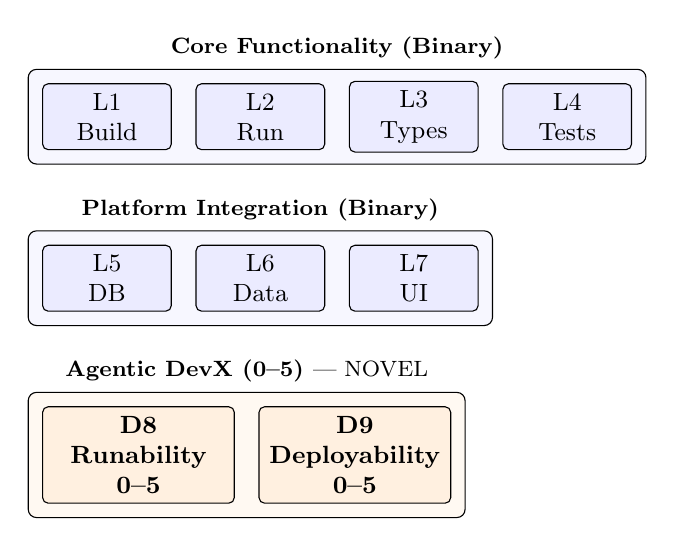
\begin{tikzpicture}[node distance=0.4cm]
  % Core Functionality
  \node[sysblock, text width=1.4cm, minimum height=0.7cm] (l1) {L1\\Build};
  \node[sysblock, text width=1.4cm, minimum height=0.7cm, right=0.3cm of l1] (l2) {L2\\Run};
  \node[sysblock, text width=1.4cm, minimum height=0.7cm, right=0.3cm of l2] (l3) {L3\\Types};
  \node[sysblock, text width=1.4cm, minimum height=0.7cm, right=0.3cm of l3] (l4) {L4\\Tests};

  \begin{scope}[on background layer]
    \node[draw, rounded corners=3pt, fill=blue!3, fit=(l1)(l4), inner sep=5pt, label={[font=\footnotesize\bfseries]above:Core Functionality (Binary)}] (core) {};
  \end{scope}

  % Platform Integration
  \node[sysblock, text width=1.4cm, minimum height=0.7cm, below=1.2cm of l1] (l5) {L5\\DB};
  \node[sysblock, text width=1.4cm, minimum height=0.7cm, right=0.3cm of l5] (l6) {L6\\Data};
  \node[sysblock, text width=1.4cm, minimum height=0.7cm, right=0.3cm of l6] (l7) {L7\\UI};

  \begin{scope}[on background layer]
    \node[draw, rounded corners=3pt, fill=blue!3, fit=(l5)(l7), inner sep=5pt, label={[font=\footnotesize\bfseries]above:Platform Integration (Binary)}] (plat) {};
  \end{scope}

  % Agentic DevX
  \node[pillarbox, text width=2.2cm, minimum height=0.7cm, below=1.2cm of l5.south west, anchor=north west] (d8) {D8\\Runability\\0--5};
  \node[pillarbox, text width=2.2cm, minimum height=0.7cm, right=0.3cm of d8] (d9) {D9\\Deployability\\0--5};

  \begin{scope}[on background layer]
    \node[draw, rounded corners=3pt, fill=orange!5, fit=(d8)(d9), inner sep=5pt, label={[font=\footnotesize\bfseries]above:Agentic DevX (0--5) \textnormal{--- NOVEL}}] (devx) {};
  \end{scope}
\end{tikzpicture}
\caption{AppEval 9-metric framework. L1--L4 check correctness, L5--L7 verify platform integration, D8--D9 (Agentic DevX) measure agent-operability---the novel contribution.}
\label{fig:appeval-framework}
\end{figure}

L1--L4 are standard software quality checks. L5--L7 verify platform integration. D8--D9 (Agentic DevX) ask the question existing frameworks miss: is this output usable in an agentic pipeline?

\subsection{Cluster-Based Quality Assessment}
\label{sec:devx-clustering}

As a weight-free alternative to composite scoring, we apply $k$-means clustering with cosine similarity on metric vectors. Each application is represented as a 9-dimensional vector $\mathbf{m} = (L_1, \ldots, L_7, \hat{D}_8, \hat{D}_9)$ where $\hat{D}_i = D_i / 5$ normalizes DevX scores to $[0,1]$. We cluster applications into quality tiers (e.g., $k=3$: low, medium, high) without requiring explicit pillar weights---the structure emerges from the data.

This approach follows~\citet{knyazev2009clustering}, who demonstrated that metric-space clustering can classify software artifacts without manual threshold tuning. For our 20-application dataset, three clusters naturally separate: (1)~applications that fail build/runtime, (2)~applications that build but lack DevX artifacts, and (3)~applications with both functional correctness and agent-operability. The cluster boundaries provide empirical quality tiers that complement the rubric-based D8/D9 scores.

\subsection{DORA Alignment}
\label{sec:devx-dora}

To ground our metrics in industry practice, we map to DORA~\cite{forsgren2018accelerate} delivery metrics:

\begin{table}[h]
\caption{DORA metric mapping.}
\label{tab:dora}
\centering
\small
\begin{tabular}{lp{5cm}}
\toprule
\textbf{DORA Metric} & \textbf{AppEval Mapping} \\
\midrule
Deployment Frequency & Successful D9 events per evaluation \\
Lead Time & Time from prompt to successful deployment \\
Change Failure Rate & Fraction of deployments failing healthcheck \\
MTTR & Time from failure to restored deployment \\
\bottomrule
\end{tabular}
\end{table}

This mapping lets teams familiar with DORA interpret our results in their existing framework.

%% ============================================================
%% 5. GENERATION--EVALUATION ISOLATION
%% ============================================================
\section{Generation--Evaluation Isolation}
\label{sec:isolation}

A critical design requirement is that the generator and evaluator must be \emph{strictly isolated}. Without isolation, the generator agent can exploit evaluation artifacts---a form of reward hacking~\cite{amodei2016concrete} that inflates metrics without improving application quality.

\subsection{Threat Model: Metric Gaming}
\label{sec:isolation-threat}

Agentic coding systems actively explore their filesystem via tools like \texttt{Read}, \texttt{Glob}, and \texttt{Grep}. When evaluation code resides in the same workspace, the following attack surfaces emerge:

\textbf{Scenario 1: Eval check reverse-engineering.} Our DB connectivity check (\texttt{eval\_checks.py:39--70})\footnote{\url{https://github.com/neondatabase/appdotbuild-agent/blob/main/klaudbiusz/cli/evaluation/eval_checks.py\#L39-L70}} verifies connectivity by calling tRPC endpoints and parsing JSON responses. An agent with read access could discover this check and create minimal stubs that pass the binary metric without implementing genuine queries:

\begin{lstlisting}[basicstyle=\ttfamily\footnotesize]
// Hypothetical stub (passes L5, no real data)
healthcheck: publicProcedure.query(() => ({
  result: { data: [], status: "ok" }
}))
\end{lstlisting}

\textbf{Scenario 2: Composite score optimization.} The evaluation weights are defined in \texttt{eval\_metrics.py}\footnote{\url{https://github.com/neondatabase/appdotbuild-agent/blob/main/klaudbiusz/cli/evaluation/eval_metrics.py\#L44-L88}}. An agent that reads this file could prioritize boilerplate (\texttt{.env.example}, \texttt{Dockerfile}) for DevX points while neglecting metrics requiring genuine implementation.

\textbf{Scenario 3: Pattern copying from prior runs.} If prior generations are accessible, an agent could copy file structures verbatim rather than reasoning about current requirements.

\subsection{Container-Level Isolation via Dagger}
\label{sec:isolation-container}

We enforce isolation at the container build level. The generation Dockerfile\footnote{\url{https://github.com/neondatabase/appdotbuild-agent/blob/main/klaudbiusz/Dockerfile\#L58-L64}} selectively copies only generation-related code:

\begin{lstlisting}[basicstyle=\ttfamily\footnotesize]
# Exclude evaluation to prevent reward hacking
COPY cli/generation/    ./cli/generation/
COPY cli/utils/         ./cli/utils/
# NOT copied: cli/evaluation/,
#             cli/analyze_trajectories.py
\end{lstlisting}

Each generation starts from a clean workspace. In bulk runs, a pre-generation directory snapshot\footnote{\url{https://github.com/neondatabase/appdotbuild-agent/blob/main/klaudbiusz/cli/generation/container_runner.py\#L76}} prevents cross-contamination between parallel generations.

%% --- TikZ Figure 5: Isolation Boundaries ---
\begin{figure}[t]
\centering
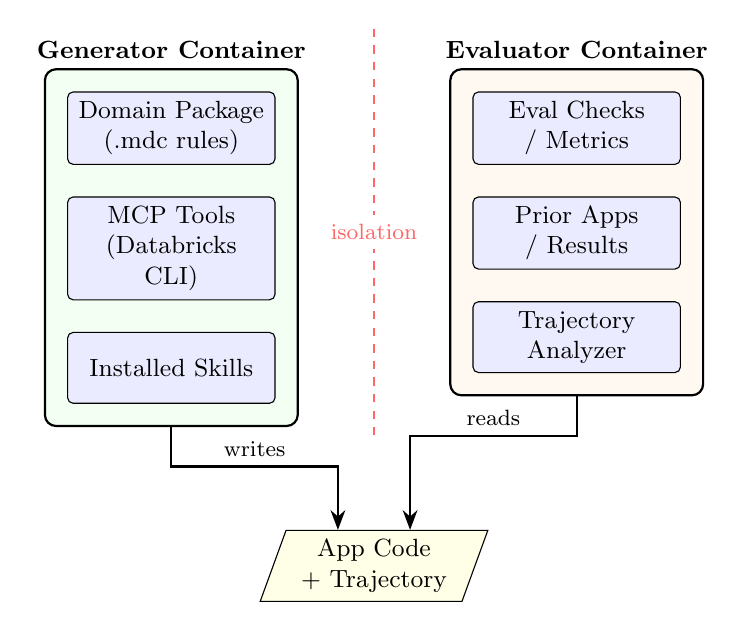
\begin{tikzpicture}[node distance=0.5cm]
  % Generator box
  \node[sysblock, text width=2.4cm] (pkg) {Domain Package\\(.mdc rules)};
  \node[sysblock, text width=2.4cm, below=0.4cm of pkg] (mcp) {MCP Tools\\(Databricks CLI)};
  \node[sysblock, text width=2.4cm, below=0.4cm of mcp] (skills) {Installed Skills};

  \begin{scope}[on background layer]
    \node[draw, thick, rounded corners=4pt, fill=green!5, fit=(pkg)(mcp)(skills), inner sep=8pt, label={[font=\small\bfseries]above:Generator Container}] (gen) {};
  \end{scope}

  % Evaluator box
  \node[sysblock, text width=2.4cm, right=2.5cm of pkg] (checks) {Eval Checks\\/ Metrics};
  \node[sysblock, text width=2.4cm, below=0.4cm of checks] (prior) {Prior Apps\\/ Results};
  \node[sysblock, text width=2.4cm, below=0.4cm of prior] (ta) {Trajectory\\Analyzer};

  \begin{scope}[on background layer]
    \node[draw, thick, rounded corners=4pt, fill=orange!5, fit=(checks)(prior)(ta), inner sep=8pt, label={[font=\small\bfseries]above:Evaluator Container}] (eval) {};
  \end{scope}

  % Shared artifacts
  \node[databox, text width=2cm, below=1.5cm of $(gen.south)!0.5!(eval.south)$] (app) {App Code\\+ Trajectory};

  \draw[arr] (gen.south) -- ++(0,-0.5) -| node[near start, above, font=\footnotesize]{writes} (app.north west);
  \draw[arr] (eval.south) -- ++(0,-0.5) -| node[near start, above, font=\footnotesize]{reads} (app.north east);

  % Barrier
  \draw[thick, dashed, red!60] ($(gen.north east)!0.5!(eval.north west)+(0,0.5)$) -- ($(gen.south east)!0.5!(eval.south west)+(0,-0.3)$) node[midway, fill=white, font=\footnotesize\color{red!60}] {isolation};
\end{tikzpicture}
\caption{Isolation boundaries between generation and evaluation. The generator cannot read evaluation code; improvements flow only through the domain package.}
\label{fig:isolation}
\end{figure}

\begin{table}[h]
\caption{Isolation boundaries between generation and evaluation.}
\label{tab:isolation}
\centering
\small
\begin{tabular}{lcc}
\toprule
\textbf{Artifact} & \textbf{Generator} & \textbf{Evaluator} \\
\midrule
Domain package (.mdc rules) & \checkmark & --- \\
MCP tools (Databricks CLI) & \checkmark & --- \\
Installed skills & \checkmark & --- \\
Evaluation checks / metrics & --- & \checkmark \\
Prior generated apps / results & --- & \checkmark \\
Trajectory analyzer & --- & \checkmark \\
Current app code & writes & reads \\
Current trajectory & writes & reads \\
\bottomrule
\end{tabular}
\end{table}

This separation mirrors training/test splits in machine learning: the generator learns from the domain package (training signal), while the evaluator measures generalization against unseen criteria. We recommend that agent evaluation frameworks enforce container-level isolation as a baseline requirement.

%% ============================================================
%% 6. RESULTS
%% ============================================================
\section{Results}
\label{sec:results}

\subsection{Generation Performance}
\label{sec:results-perf}

We evaluated on 20 Databricks applications spanning dashboards, analytics tools, and business intelligence interfaces. Each app was generated from a natural language prompt describing the desired functionality.

\begin{table}[h]
\caption{Aggregate evaluation results ($n=20$ applications).}
\label{tab:results}
\centering
\small
\begin{tabular}{llcc}
\toprule
\textbf{ID} & \textbf{Metric} & \textbf{Result} & \textbf{Notes} \\
\midrule
L1 & Build Success & 18/20 (90\%) & \\
L2 & Runtime Success & 18/20 (90\%) & \\
L3 & Type Safety & 1/20 (5\%) & Primary gap \\
L5 & DB Connectivity & 18/20 (90\%) & \\
D8 & Runability & 3.0/5 avg & \\
D9 & Deployability & 2.5/5 avg & \\
\bottomrule
\end{tabular}
\end{table}

The 90\% build/runtime success indicates the core generation pipeline works. The 5\% type safety rate is the primary gap---trajectory analysis traced this to TypeScript strict mode violations, particularly null handling.

\subsection{Efficiency}
\label{sec:results-efficiency}

Generation is practical for real use: under 10 minutes and under \$1 per application.

\begin{table}[h]
\caption{Efficiency metrics ($n=20$ applications).}
\label{tab:efficiency}
\centering
\small
\begin{tabular}{lcc}
\toprule
\textbf{Metric} & \textbf{Value} & \textbf{Notes} \\
\midrule
Generation Time & 6--9 min & End-to-end \\
Cost per App & \$0.74 & API cost \\
Agent Turns & 93 avg & Conversation turns \\
Lines of Code & 732 avg & Generated LOC \\
\bottomrule
\end{tabular}
\end{table}

Cost is dominated by the reasoning model (Claude Sonnet). The 93 turns include data exploration, scaffolding, iterative code generation, and validation.

\subsection{Feedback Loop in Action}
\label{sec:results-loop}

The trajectory analyzer identified type safety as the primary gap (5\% pass rate). Root cause from trajectory analysis: TypeScript strict mode violations, particularly null handling in generated code.

This demonstrates the feedback loop:
\begin{enumerate}
    \item Agents used the package $\to$ generated apps with type errors
    \item Trajectories showed repeated \texttt{tsc} failures and confusion about null checks
    \item Analyzer recommended: add explicit null handling examples to CLAUDE.md guidance
    \item Fix implemented $\to$ next iteration showed improvement
\end{enumerate}

%% ============================================================
%% 7. RELATED WORK
%% ============================================================
\section{Related Work}
\label{sec:related}

\textbf{Environment matters more than model.} Recent work~\cite{kniazev2025appbuild} compared agent performance across different environments. Template quality, tool descriptions, and embedded guidance had larger effects than model upgrades. This motivates the focus on improving tooling rather than agents.

\textbf{Evaluation gap.} Existing benchmarks evaluate code correctness (HumanEval~\cite{chen2021evaluating}, SWE-bench~\cite{jimenez2024swe}), task completion (WebArena~\cite{zhou2024webarena}, GAIA~\cite{mialon2023gaia}), or SQL quality (BIRD~\cite{bird2023}, Spider~\cite{yu2018spider}). None ask whether generated code can be operated by other agents---a critical question for compound AI systems where one agent's output becomes another's input.

\textbf{Agent tool protocols.} The Model Context Protocol (MCP) standardizes agent-tool interaction. Cloudflare~\cite{cloudflare2024codemode} and Anthropic~\cite{anthropic2024tools} report that LLMs perform better writing code to call tools than calling tools directly. We adopt this pattern.

\textbf{Trajectory analysis.} Analyzing agent execution traces for debugging is established practice (SWE-agent~\cite{yang2024swe}, OpenHands~\cite{wang2024openhands}). Our contribution is making the synthesis phase itself agentic---an agent that explores source code to generate recommendations, rather than static aggregation.

\textbf{Agent evaluation harnesses.} Inspect AI~\cite{inspectai2024} and DeepEval~\cite{deepeval2024} provide evaluation infrastructure but focus on correctness rather than deployment readiness. AgentBench~\cite{agentbench2023} spans multiple environments but does not evaluate autonomous deployability.

%% ============================================================
%% 8. DISCUSSION
%% ============================================================
\section{Discussion}
\label{sec:discussion}

\subsection{Agent-Agnostic vs Agent-Specific}
\label{sec:disc-agnostic}

Our approach invests in tooling rather than agents. This is a deliberate bet: agents improve rapidly (model upgrades are free to adopters), while domain knowledge is slow to encode and hard to transfer. By packaging knowledge as installable artifacts, we ensure that every agent improvement automatically benefits users without re-implementation.

The tradeoff is control. Agent-specific approaches can fine-tune behavior precisely; our agent-agnostic design relies on the agent's ability to follow tool descriptions and guidance. In practice, we find this sufficient for structured tasks (scaffolding, validation, deployment) but limiting for open-ended reasoning about application architecture.

\subsection{The DevX Dimension}
\label{sec:disc-devx}

Agentic DevX introduces a genuinely new evaluation dimension. Existing benchmarks implicitly assume a human operator who can bridge gaps between generated code and running software. As AI systems become compound---with agents consuming other agents' outputs---this assumption breaks down.

We argue that DevX metrics will become increasingly important as agent pipelines deepen. A code generation agent whose output cannot be operated by a deployment agent is only partially useful, regardless of code quality.

\subsection{Limitations}
\label{sec:disc-limitations}

\textbf{Platform specificity.} We validate on Databricks; the architecture generalizes but requires platform-specific implementation work.

\textbf{Dataset size.} Twenty applications provide initial validation; scaling to 100+ is planned.

\textbf{Type safety gap.} The 5\% pass rate indicates template/guidance issues. The trajectory analyzer identified the cause; fixes are being validated through subsequent loop iterations.

\textbf{Agentic DevX validation.} Current scores are proxy measurements based on artifact presence; future work should validate with actual agent operation trials.

\textbf{Loop maturity.} We run the feedback loop continuously; reported results reflect multiple iterations. A longer-term longitudinal study would strengthen confidence in the approach.

\subsection{Broader Implications}
\label{sec:disc-broader}

The feedback loop pattern---generate, analyze trajectories, improve tooling, re-evaluate---is not specific to Databricks or even to code generation. Any domain where agents use tools to produce artifacts can benefit from trajectory-based tooling improvement. The key insight is that agent failures are often environmental failures in disguise, and the fix is better infrastructure rather than better models.

By establishing standardized metrics for autonomous operability, we enable reproducible benchmarking, objective comparison across approaches, and systematic improvement through trajectory-based feedback.

%% ============================================================
%% 9. CONCLUSION
%% ============================================================
\section{Conclusion}
\label{sec:conclusion}

We presented a feedback loop for iterative improvement of agent tooling:

\begin{enumerate}
    \item \textbf{Installable domain knowledge} packages expertise as agent-consumable artifacts
    \item Agents use the package, producing \textbf{trajectories}
    \item \textbf{Agentic trajectory analyzer} identifies friction and recommends fixes
    \item \textbf{Agentic DevX metrics} verify the final output is agent-operable
\end{enumerate}

When agents fail, improve their environment rather than the agents themselves. Our system operationalizes this insight with a closed loop---trajectories reveal friction, analysis produces fixes, evaluation verifies improvement.

On 20 Databricks applications across multiple agent backends, we achieve 90\% build success at \$0.74/app. The trajectory analyzer identified concrete improvements that we implemented and verified, demonstrating the loop in practice.

\textbf{Open source.} Domain package, trajectory analyzer, and evaluation harness available at: [URL redacted for review]

%%
%% Acknowledgments (hidden for review)
%%
% \begin{acks}
% Supported by Neon and Databricks.
% \end{acks}

%%
%% Bibliography
%%
\bibliographystyle{ACM-Reference-Format}
\bibliography{references}

\end{document}
